\chapter{Analysis and Experiments}

\section{Analysis}
\section{Experiments}
%0. what are you going to do.
%
%1. how did you do this? *********
%
%2. give an example.
%
%3. what did you find?
%
%4. conclusion.

In this section, we analyze how CueNet drives a real world face tagging application. The application contains a set of photos, and a database of people, and its goal is to associate the right persons for each photo, with high accuracy. The goal of CueNet, and the focus of our analysis, is to provide small search spaces so that the application can exhibit high accuracy in all datasets.

In the following evaluation, we investigate three hypotheses. \textbf{First}, what sources provide the most interesting context? \textbf{Second}, how small are the candidates lists constructed by the discovery algorithm, which are provided to the classification algorithm as a ``pruned" version of the search space? And \textbf{third}, what percentage of true positives does this pruned search space contain?

\subsection{Setup}
We use 368 photos taken at 7 different conferences in our face tagging experiment. The person database consists of 660 people. Each photo contains one or more persons from this database. The owner of the photos was asked to provide access to their professional Google Calendar to access personal events. Information from social networks was gathered. Specifically, events, social graph, photos of user and their friends from Facebook. In order to obtain information of the conference event, we used the Stanford NER\cite{finkel2005incorporating} to extract names of people from the conference web pages. Descriptions of the keynote, session and banquet events were manually entered into the database. Our sources also included personal emails, access to public events website upcoming.com (Yahoo! Upcoming) and used Yahoo! PlaceFinder for geocoding addresses.

The ground truth was annotated by the user with our annotation interface. For each photo, this essentially consisted of the ID of the persons in it.  We will denote each dataset as `Di' (where 1 $\leq$ $i$ $\leq$ 8 for each dataset). Table \ref{tbl:unique-persons} describes each dataset in terms of number of photos, unique annotations in ground truth and the year they were captured. The total number of unique people who could have appeared in any photo in our experiments is 660. This set forms the exhaustive search space, $L$ from section \ref{sec:first-k}.

\begin{table}[h]
\begin{center}
\begin{tabular}{ |c|p{1.5cm}|p{1.5cm}|c| }
  \hline
  \texttt{Dataset} & \texttt{Unique People} & \texttt{No.\ of Photos} & \texttt{Year} \\
  \hline
%  D0 & TBD & TBD & 2009\\
  D1 & 43 & 78 & 2012\\
  D2 & 24 & 108 & 2012\\
  D3 & 6 & 16 & 2010\\
  D4 & 7 & 10 & 2010\\
  D5 & 36 & 80 & 2009\\
  D6 & 18 & 65 & 2013\\
  D7 & 7 & 11 & 2013\\
  \hline
\end{tabular}
\caption{Profile of datasets used in the experiments.}
\label{tbl:unique-persons}
\end{center}
\end{table}

We divide the sources into different categories to facilitate a more general discussion. The categories are ``Personal Information" (same as Owner Information in section \ref{sec:discovery-algorithm}), ``Event sources", and ``Social Networks". Event sources include Facebook events, Yahoo Upcoming web service, our conference events database among other sources. Social networks include Facebook's social graph. Personal information contained information about the user, and a link to their personal calendars. An annotation is considered ``Out of Context Network" if it is not in any of these sources.

\begin{figure}[t]
\centering
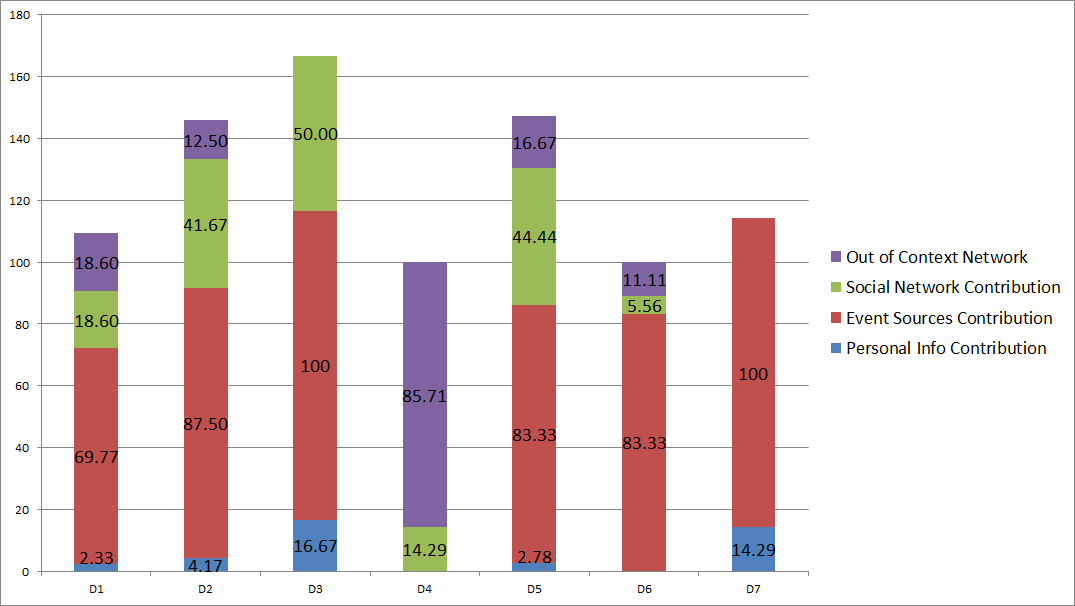
\includegraphics[width=0.9\textwidth]{media/gt-distro-stacked-2.png}
\caption{The distribution of annotations in the ground truth across various sources.}
\label{fig:src-cand-distribution}
\end{figure}

Figure \ref{fig:src-cand-distribution} shows the distribution of the ground truth annotations across various sources, for each dataset. For example, the bar corresponding to D2 says that 87.5\% of ground truth annotations were found in event sources, 41.67\% in social networks, 4.17\% in personal information and 12.5\% were not found in any source, and therefore marked as ``Out of Context Network". From this graph it is clear that event sources contain a large portion of ground truth annotations. Besides D4, a minimum of 70\% of our annotations are found in event sources for all datasets, and for some datasets (D3, D7) all annotations are found in event sources. The sum total of contributions will add up to values more than 100\% because they share some annotations among each other. For example, a friend on Facebook might show up at a conference to give the keynote talk.

\subsection{Context Discovery}
Now, lets look at reduction obtained in state space with the discovery algorithm. The total number of people in our experiment universe is 660. By statically linking the sources, we would expect the search space to contain 660 candidates for tagging any of the datasets. However, the context discovery algorithm reduced the size of the search space as shown in table \ref{tbl:search-spaces}. The search space varies from 7 people in D7 (1\%) to 338 people in D2 (51\%). We denote the term hit rate as the percentage of true positives in the search space. Even if our search space is small, it might contain no annotations from the ground truth, leading to poor classifier performance. The hit rates are also summarized in table \ref{tbl:search-spaces}. For D4, the algorithm found no event sources (as seen in figure \ref{fig:src-cand-distribution}), and therefore constructed a search space which was too small, thereby containing none of the ground truth. With the exception for D4, the hit rate is always above 83\%. We observe an overall reduction in the search space size, with a high hit rate for majority of the datasets. 

\begin{table}[h]
\begin{center}
\begin{tabular}{ |c|p{2.5cm}|c| }
  \hline
  \texttt{Dataset} & \texttt{Reduced Search Space Size} & \texttt{Hit Rate}\\
  \hline
%  D0 & TBD & TBD \\
  D1 & 42 & 83.72\%\\
  D2 & 338 & 87.5\%\\
  D3 & 231 & 100\%\\
  D4 & 1 & 0\%\\
  D5 & 254 & 83.33\%\\
  D6 & 20 & 88.89\%\\
  D7 & 7 & 100\%\\
  \hline
\end{tabular}
\caption{Sizes of Search Space for each dataset.}
\label{tbl:search-spaces}
\end{center}
\end{table}

We now investigate the role of different context sources in the discovery algorithm. If an entity in the search space was merged into the event graph by an event source, they are said to be ``contributed" from it. We profiled our algorithm to log all contributions which were true positives for the classification algorithm. Figure \ref{fig:tag-distribution} shows the contribution from various sources for all datasets. For example, D1 obtained 69.77\% of true positives in its search space from event sources, 2.33\% from personal information and 11.63\% from social networks. 16.28\% of true positives for D1 were obtained from no source, and were therefore marked as ``Out of Context Network". 

This graph brings to light our argument that most of the true positives, for all datasets, were obtained as a result of navigating the event sources. It will also be noted that the role of social networks is minimal. It was found useful for only one dataset. Relying on social networking sources would have led to a large number of false positives in the classifier performance. Even though the role of personal information is negligible, it is critical in linking in photos to the owner, and from there to different events. Without the availability of personal information, the algorithm would not have reached the context rich event sources.

% the lower selection of candidates shows the selectivity of CueNet in extracting information from different sources. Because it constructs queries with as many predicates as possible, the availability of time and space prompts it to navigate event sources more than social networking sources.

\begin{figure*}[t]
\centering
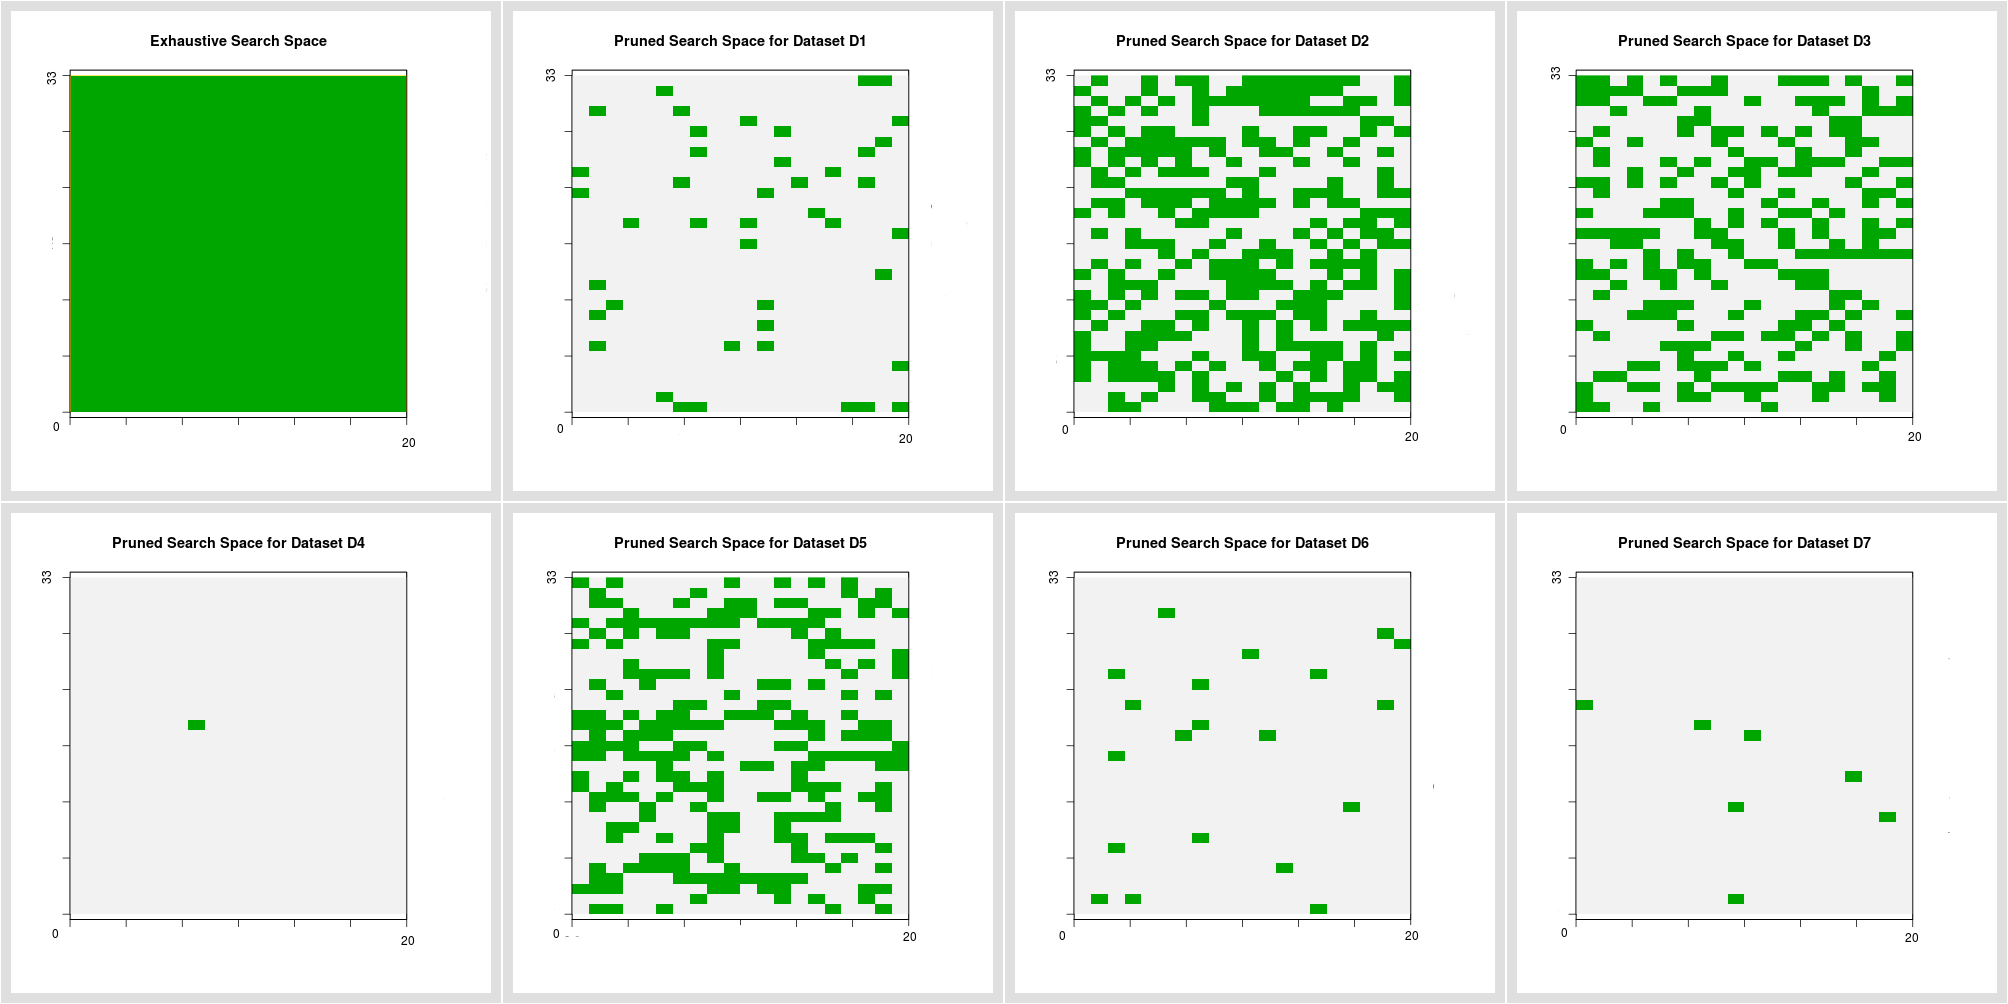
\includegraphics[width=\textwidth]{diversity/montage-clean-pruned-labelled.png}
\caption{Grid plots showing the exhaustive search space and pruning in search space for different datasets.}
\label{fig:diversity}
\end{figure*}

\subsection{Individual List Sizes in a Dataset}
Here we look at how CueNet reduces the number of possible candidates for all photos in a dataset. For this setup, the complete candidate set $L$, contained 1894 labels (total number of people present at the conference, user's emails and social graph). The figure \ref{fig:exp-vldb-all-cx} shows various statistics for each photo, which includes the maximum size of the list which was generated by the discovery algorithm, the actual number of people in the photos, the number of true positives and false positives. As it can be seen, the size of the discovered set $S$, never exceeded 12. This is 0.5\% of the original candidate list. Because the total number of possible participants (list size) was low, our False Positive rate (FP) was very low too. Most of the false positives were due to profile orientation of faces or obstructions (this was because the face detector was smart enough to pick up profile faces, but verification worked better only on frontal faces).

\begin{figure}[t]
\centering
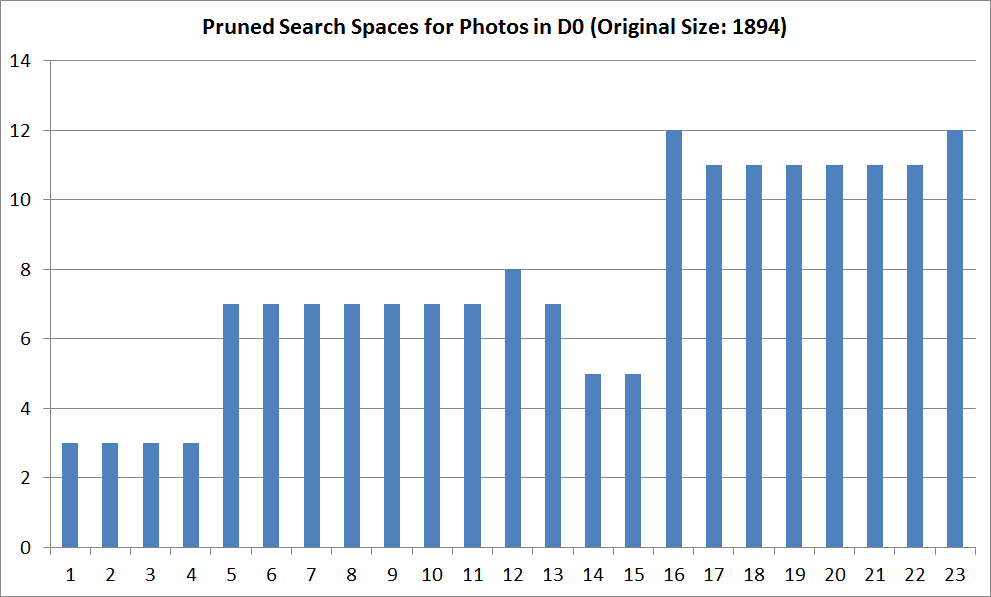
\includegraphics[width=0.9\textwidth]{media/reduced-list-sizes-d0.png}
\caption{Pruned search space for photos in D0.}
\label{fig:exp-vldb-all-cx}
\end{figure}

\subsection{Search Spaces}
Finally, we compare the various search spaces constructed by discovery algorithm. We represent all people in our experiment universe in a color grid (with 33x20 cells for 660 people). Each cell represents the presence or absence of a person in the search space. If a person was present in the candidate list provided to the tagging algorithm, we color the corresponding cell green, otherwise it is colored white. Figure \ref{fig:diversity} shows the color grids describing search spaces for all datasets, and an exhaustive search space. The positioning of people along the grid is arbitrary, but consistent across grids. Our aim in this visualization is to see the diversity in search spaces created by the algorithm. The purpose of the exhaustive search space is to provide easy comparision to appreciate the reduction in search space. 

It can be seen that CueNet prunes the search space very differently for different datasets. As we move from dataset to dataset, the data sources present different items of information, and therefore CueNet constructs very search spaces. Dataset D2, D4 and D5 are very large conferences hosting hundreds of people in the same field. This explains why a large portion of the grid is covered. Also, this was the same conference held in three different years, and therefore, had a lot of common attendees resulting in overlap.

\subsection{Conclusion}
These experiments validate our three hypotheses. \textbf{First}, Event sources contain a large portion of true positives. From 70\% in D1 to 100\% in D7. There are events for which there is no documentation, and event sources are not able to contribute anything here, as in the case of D4. \textbf{Second}, the discovery algorithm is able to prune the search space using event, personal and social information. The reduction is atleast 50\% for D2 (338 candidates out of 660) but can be very large in some cases (7 candidates for D7). \textbf{Third}, The reduced search space retains a high number of true positives. The hit rate is between 83\% to 100\% (with the exception of D4, where the search space provided no true positives). We also saw how unique the search spaces are, to each dataset, thereby demonstrating the dynamic nature of the algorithm.

\begin{figure}[t]
\centering
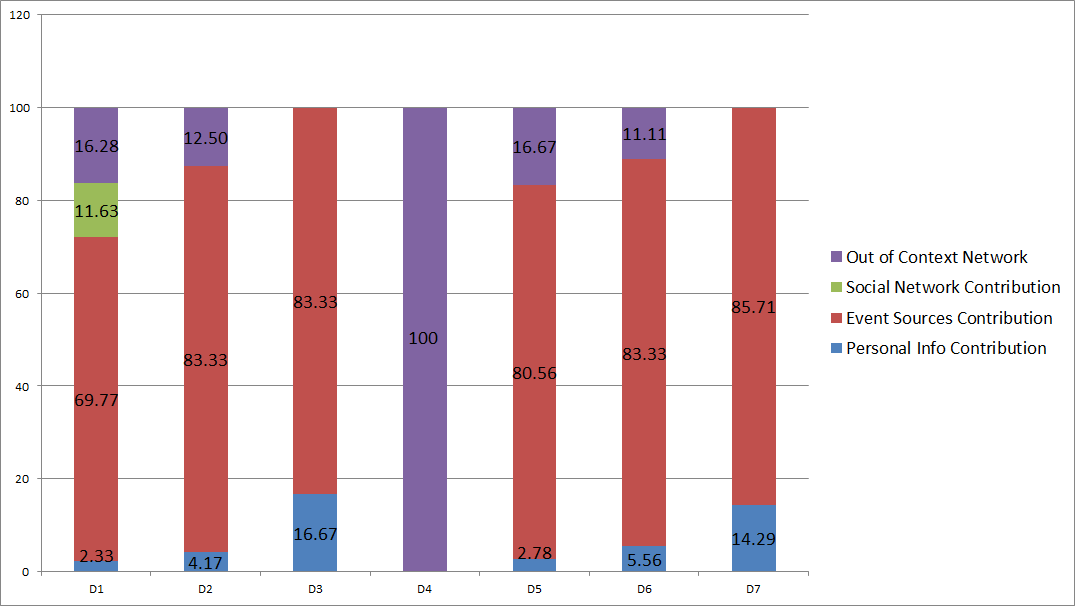
\includegraphics[width=0.9\textwidth]{media/discovery-distro-stacked-2.png}
\caption{Graph showing the contribution of each source type in context discovery.}
\label{fig:tag-distribution}
\end{figure}

\section{Known Issues}
In this section, we list some of the issues encountered in designing and building CueNet. Some of these are active areas of research, and whereas others are specific to our framework, and can be considered potential areas of research. Our experience with CueNet indicates that the following issues should be approached in a holistic manner, i.e., in conjunction with each other. Approaching these problems in the context of each other reduces the individual complexity of each sub-problem by possibly increasing the complexity of the entire framework, but making the problem more tractable.

\textbf{\textbf{Noise in Social Media}}: The problem of noise filtering in web data is a prominent one, and is being addressed by various communities in different ways. These range from entity matching and record linkage problems \cite{elmagarmid2007duplicate} to correcting missing data in information networks \cite{sadikov2011correcting}. These problems get trickier because of the different variations in representing tiny details such as representation names of people, addresses of places, and time. In fact, there is a whole school of anthroponomastics \cite{schneider2009s} dedicated to studying variations in human names. Ideas in this field indicate that these differences arise due to cultural, historical and environmental issues\cite{al2009socio}. Such issues cannot be trivially addressed. 

%Consider, for example, the Hebrew name below:
%
%\begin{figure}[h]
%\centering
%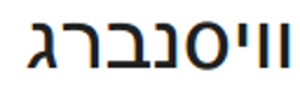
\includegraphics[width=0.15\textwidth]{media/ronen.png}
%\label{fig:exp-general-loc-cx}
%\end{figure}
%
%It can be translated to English as ``Waisenberg" or ``Vaisenberg". So are Mr.\ X Waisenberg who authored a paper in a Security conference and Dr.\ X Vaisenberg who works at Google, the same person? They might be if X has semitic origins!

Face tagging in social media sources like Facebook can also be very noisy. This strictly prohibits directly using this data to train verification/recognition models. Also, the quality of photos are poor, resulting in weaker features, which would have otherwise allowed better matching. 

An exhaustive scientific characterization of noise in social media is beyond the scope of this paper, and is being investigated step by step in social media research communities.

\textbf{\textbf{CPU Efficiency}}: The query engine in CueNet is responsible for extracting data from different sources. If a very large number of photos are being tagged, our scheme of query generation and merging will prove inefficient. Processing many photos from different people provides a very rich opportunity to develop interesting heuristics using event semantics for the multi-query optimization problem. Also, partitioning the discovery algorithm such that the computations can occur in a distributed manner is a complex problem. Such steps will be required if the application workload is of the scales of Facebook or processing photos in real time at the scales of Instagram.

\textbf{\textbf{Face Verification}}: Even though face recognition has been studied in research for the last two decades, face verification, and its specific application to faces in the wild has been a relatively recent venture. Although the accuracy of these systems is commendable, the problems of occlusion, image quality, face alignment and differing lighting conditions exist. These hard problems need to be solved before ``perfect" or ``near-perfect" verification can be established. 

\textbf{\textbf{Execution Patterns}}: When is a good time to execute the algorithm? When a user takes a photo? Or before she uploads it to her favorite photo sharing site? For the current evaluation, contextual sources are assumed to be immutable. This is not true in the real world. Contextual sources are constantly being appended with new information, and old information is being updated. These updates may be vital in tagging a certain photo. So the question of when to execute the algorithm, or how and when to query the sources is an open question. If a large number of photos are to be tagged, and a busy source like Facebook is being used for context, the CueNet query engine must take into account various freshness metrics and crawling policies of the sources. 

\textbf{\textbf{Open Datasets}}: The unavailability of a large public data set over which different techniques can be evaluated against each other is an open problem. As seen in our experiments, personal information is vital to contextual approaches, and this data is largely personal, and therefore cannot be shared openly. Optimal anonymization techniques need be to invented such that the privacy of the experiment participants are maintained, and at the same time the data is meaningful to be applied in contextual approaches to problems. This need to be solved so that new context discovery techniques can be evaluated independently and against each other, over a common platform.